\documentclass[10pt, USenglish]{beamer}

\usepackage[T1]{fontenc}
\usepackage[utf8]{inputenc}
\usepackage{lmodern}
\usepackage{graphicx}

\usepackage{amssymb}

\usepackage{babel}
\usepackage{mathtools}
\usepackage{IEEEtrantools}

\usepackage{esvect}

% Operator Deklarationen
\DeclareMathOperator{\curl}{rot}
\DeclareMathOperator{\grad}{grad}
\DeclareMathOperator{\dive}{div}
\DeclareMathOperator{\supp}{supp}

\DeclareMathOperator{\dist}{dist}

\newcommand{\lapl}{\Delta}
% Symbols
\newcommand{\projP}{\mathbb{P}}
\newcommand{\polyP}{\mathbb{P}}
\newcommand{\meshT}{\mathcal{T}}
\newcommand{\Shp}{\mathcal{S}_h^p}
\newcommand{\intfI}{\mathcal{I}}
\newcommand{\distT}{\mathcal{T}}
\newcommand{\adj}{*}
\newcommand{\sip}{{\mathrm{sip}}}

\newcommand{\markvec}[1]{\vv{#1}}

% Operators
\newcommand{\lavg}{\langle\!\langle}
\newcommand{\ravg}{\rangle\!\rangle}
%\DeclarePairedDelimiter{\}
\newcommand{\ljump}{{\lbrack\!\lbrack}}
\newcommand{\rjump}{{\rbrack\!\rbrack}}
\newcommand{\lupw}{{\{\!\!\{}}
\newcommand{\rupw}{{\}\!\!\}}^{\mathrm{up}}}
\newcommand{\ldwnd}{{\{\!\!\{}}
\newcommand{\rdwnd}{{\}\!\!\}}^{\mathrm{down}}}
\newcommand{\lDG}{\|}
\newcommand{\rDG}{\|_{\mathrm{DG}}}
\newcommand{\lDGs}{\|}
\newcommand{\rDGs}{\|_{\mathrm{DG,*}}}
\newcommand{\lDGw}{\|}
\newcommand{\rDGw}{\|_{\widetilde{\mathrm{DG}}}}

\newcommand{\diffd}{\ensuremath{\mathrm{d}}}
\newcommand{\dd}{\:\diffd}

\newcommand{\gmid}{\mathrel{}\middle|\mathrel{}}
\newcommand{\midcolon}{\mathrel{}:\mathrel{}}

% Theme Definitionen
\usetheme{Luebeck}
\usecolortheme{beaver}
\usefonttheme{professionalfonts}
\beamertemplatenavigationsymbolsempty

% Titel
\title{Space-time dG methods for parabolic optimal control problems}
\date{15. December 2016}
\institute{Universität Bonn}
\author{Christian Pfeiffer}

\begin{document}

% Titelfolie
\begin{frame}
	\titlepage
\end{frame}

% Inhaltsverzeichnis
\begin{frame}
	\frametitle{Space-time discontinuous Galerkin methods for parabolic optimal control problems}
	\framesubtitle{Overview}
	\tableofcontents[hideallsubsections]
\end{frame}

\section{A space-time dG method for the parabolic heat equation}

\subsection{Problem formulation}

\begin{frame}
\begin{itemize}
\item Parabolic heat equation:
\[
\begin{IEEEeqnarraybox}[][c]{rCl"l}
\frac{\partial f}{\partial t} (x, t) - \lapl f(x, t) &=& g_I(x, t) & \text{for } (x, t) \in \Omega, \\
f(x, t) &=& 0 & \text{for } (x, t) \in \Sigma_D, \\
n_x(x,t) \cdot \nabla_x f(x, t) + \alpha f(x, t) &=& g_R(x, t) & \text{for } (x, t) \in \Sigma_R, \\
f(x, 0) &=& f_0(x) & \text{for } (x, t) \in \Omega.
\end{IEEEeqnarraybox}
\]
\item Need to discretize $\partial_t f$ and $\lapl f$.
\item Function space to work with:
\begin{IEEEeqnarray*}{r}
	\IEEEeqnarraymulticol{1}{l}{ \Shp(\meshT_N) \coloneqq \left\{ v_h \in L_2(Q) \gmid v_h |_{\tau_\ell} \in \polyP_p(\tau_\ell) \text{ for all } \tau_\ell \in \meshT_N \right. \qquad } \\
	\left. \text{ and } v_h = 0 \text{ on } \Sigma_D \right\}.
\end{IEEEeqnarray*}
\end{itemize}
\end{frame}

\subsection{Discretization}

\begin{frame}
\begin{itemize}
\item For treating $\lapl f$: Symmetric Interior Penalty (SIP) method.
\[
\begin{IEEEeqnarraybox}[][c]{rCl}
	a^\sip(f_h, v_h) &\coloneqq& \sum_{\ell = 1}^N \iint_{\tau_\ell} \nabla_x f_h(x, t) \cdot \nabla_x v_h(x, t) \dd x \dd t \\
	&& {} - \sum_{\Gamma_{k\ell} \in \intfI_N} \iint_{\Gamma_{k \ell}} \lavg \nabla_x f_h \ravg_{\Gamma_{k \ell}} (x, t) \ljump v_h \rjump_{\Gamma_{k \ell}, x} (x, t) \dd s \dd t \\
	&& {} - \sum_{\Gamma_{k\ell} \in \intfI_N} \iint_{\Gamma_{k \ell}} \ljump f_h \rjump_{\Gamma_{k \ell}, x} (x, t) \lavg \nabla_x v_h \ravg_{\Gamma_{k \ell}} (x, t) \dd s \dd t \\
	&& {} + \sum_{\Gamma_{k \ell} \in \intfI_N} \frac{\sigma}{\bar{h}_{k\ell}} \iint_{\Gamma_{k \ell}} \ljump f_h \rjump_{\Gamma_{k \ell}, x} \cdot \ljump v_h \rjump_{\Gamma_{k \ell}, x} \dd s \dd t.
\end{IEEEeqnarraybox}
\]
\item Hereby we denote:
\begin{itemize}
\item The jump in space direction will be denoted by
\[
	\ljump v \rjump_{\Gamma_{k \ell}, x} (x, t) \coloneqq \left. v \right|_{\tau_k} (x, t) \cdot \markvec{n_{k, x}} + \left. v \right|_{\tau_\ell} (x, t) \cdot \markvec{n_{\ell, x}} \quad \text{for } (x, t) \in \Gamma_{k, \ell}.
\]
\item The average of $v$ on the interface is going to be denoted as
\[
	\lavg v \ravg_{\Gamma_{k \ell}} (x, t) \coloneqq \frac{1}{2} \left[ v|_{\tau_k} (x, t) + v|_{\tau_\ell}(x, t) \right] \quad \text{for } (x, t) \in \Gamma_{k, \ell}.
\]
\end{itemize}
\end{itemize}
\end{frame}

\begin{frame}
\begin{itemize}
\item For the treatment of $\partial_t f$: upstream approach.
\begin{IEEEeqnarray*}{rCl}
	b(f_h, v_h) &\coloneqq& - \sum_{\ell = 1}^N \iint_{\tau_\ell} f_h(x, t) \frac{\partial v_h}{\partial t}(x, t) \dd x \dd t \\
	&& {} + \int_{\Omega} f_h(x, T) v_h(x, T) \dd s \\
	&& {} + \sum_{\Gamma_{k\ell} \in \mathcal{I}_N} \iint_{\Gamma_{k \ell}} \lupw f_h \rupw_{\Gamma_{k \ell}} (x, t) \ljump v_h \rjump_{\Gamma_{k \ell}, t} (x, t) \dd s \dd t.
\end{IEEEeqnarray*}
\item Notation:
\begin{itemize}
\item For the jump in time direction we write
\[
	\ljump v \rjump_{\Gamma_{k \ell}, t} (x, t) \coloneqq \left. v \right|_{\tau_k} (x, t) \cdot n_{k, t} + \left. v \right|_{\tau_\ell} (x, t) \cdot  n_{\ell, t} \quad \text{for } (x, t) \in \Gamma_{k, \ell}.
\]
\item The so called upwind in time direction is defined by
\[
	\lupw v \rupw_{\Gamma_{k \ell}} (x, t) \coloneqq \begin{cases}
	v|_{\tau_k}(x, t) & \text{for } n_{k, t} > 0, \\
	0 & \text{for } n_{k, t} = 0,\\
	v|_{\tau_\ell}(x, t) & \text{for } n_{k, t} < 0,
	\end{cases} \quad \text{for } (x, t) \in \Gamma_{k \ell}.
\]
\end{itemize}
\end{itemize}
\end{frame}

\subsection{Properties}

\begin{frame}
\begin{itemize}
\item Unique solution under some regularity assumptions on the mesh.
\item $b(v_h, f_h)$ discretizes $- \partial_t f$ instead of $\partial_t f$.
\item If the mesh is quasi uniform: Error estimates in an energy norm $\lDG \cdot \rDG$ if $f \in H^s(\meshT_N)$ with $s > 3/2$, where
\begin{IEEEeqnarray*}{rCl}
\| f \|_A^2 &\coloneqq& \sum_{\ell = 1}^N \| \nabla_x f \|_{[L^2(\tau_\ell)]^d}^2 + \sum_{\Gamma_{k \ell} \in \mathcal{I}_N} \frac{\sigma}{\bar{h}_{k \ell}} \left\| \ljump f \rjump_{\Gamma_{k \ell}, x} \right\|_{[L^2(\Gamma_{k \ell})]^d}^2, \\
\| f \|_B^2 &\coloneqq& \sum_{\ell = 1}^N h_\ell \| \partial_t f \|_{L^2(\tau_\ell)}^2 + \| f(0) \|_{L^2(\Omega)}^2 + \| f(T) \|_{L^2(\Omega)}^2 \\
&& + \sum_{\Gamma_{k \ell} \in \mathcal{I}_N} \left\| \ljump f \rjump_{\Gamma_{k \ell}, t} \right\|_{L^2(\Gamma_{k \ell})}^2, \\
\lDG f \rDG^2 &\coloneqq& \| f \|_A^2 + \alpha \| f \|_{L^2(\Sigma_R)}^2 + \| f \|_B^2.
\end{IEEEeqnarray*}
\end{itemize}
\end{frame}

\begin{frame}
\begin{itemize}
\item If the function is in $H^s(\meshT_N)$ with $s \geq 2$:
\[
	\lDG f - f_h \rDG \leq C \max\{ 1, \alpha \} h^{\min \{ s, p+1\} -1} |f|_{H^s(\meshT_N)}.
\]
\item Reason for requiring $s \geq 2$: Need to estimate $\| \nabla_x(f - Q_\ell f) \|_{[L^2(\partial \tau_\ell)]^d}$.
\item Under assumption of at least $H^2$ regularity for general right hand sides: 
\[
	\| f - f_h \|_{L^2(Q)} \leq C \max\{ 1, \alpha \} h^{\min \{ s, p+1\}} |f|_{H^s(\meshT_N)}.
\] 
\end{itemize}
\end{frame}

\section{Application to parabolic optimal control problems}

\subsection{The optimal control problem}

\begin{frame}
\begin{itemize}
\item Boundary optimal control formulation:
\begin{IEEEeqnarray*}{c}
\min J(y, u) = \frac{1}{2} \int_\Omega \left( y(x, T) - y_\Omega(x) \right)^2 \dd x + \frac{\lambda}{2} \iint_\Sigma u(x, t)^2 \dd s \dd t \\
\noalign{\noindent subject to\vspace{\jot}}
\begin{IEEEeqnarraybox}[][c]{rCl"l}
\frac{\partial y}{\partial t} - \lapl y &=& 0 & \text{in } Q \coloneqq \Omega \times (0, T) \\
\partial_\nu y + \alpha y &=& \beta u & \text{in } \Sigma \coloneqq \partial \Omega \times (0, T) \\
y(x, 0) &=& y_0(x) & \text{in } \Omega
\end{IEEEeqnarraybox} \\
\noalign{\noindent and\vspace{\jot}}
u_a(x, t) \leq u(x, t) \leq u_b(x, t) \quad \text{a.e.\ in $\Sigma$}.
\end{IEEEeqnarray*}
\item Alternative formulations possible, including
\begin{itemize}
\item the control operating as interior heat source,
\item the desired state being given on $Q$.
\end{itemize}
\end{itemize}
\end{frame}

\subsection{Continuous solutions}

\begin{frame}
\begin{itemize}
\item Control-to-state operator $S$ mapping $u \mapsto y(\cdot, T)$.
\item Reduced formulation:
\[
\min_{u \in U_{ad}} J(u) \coloneqq \frac{1}{2} \| S u - z \|_{L^2(\Omega)}^2 + \frac{\lambda}{2} \| u \|_{L^2(\Sigma)}^2.
\]
\item Problem possesses a unique solution $\bar{u} \in U_{ad}$.
\item A element $\bar{u} \in U_{ad}$ is optimal if and only if
\[
	\langle S \bar{u} - z, S ( u - \bar{u} ) \rangle_{L^2(\Omega)} + \lambda \langle \bar{u}, u - \bar{u} \rangle_{L^2(\Sigma)} \geq 0 \quad \text{for all } u \in U_{ad}.
\]
\end{itemize}
\end{frame}

\begin{frame}
\begin{itemize}
\item Adjoint state $p$ defined by
\[
\begin{IEEEeqnarraybox}[][c]{rCl"l}
-\frac{\partial p}{\partial t} (x, t) - \lapl p(x, t) &=& 0 & \text{for } (x, t) \in Q, \\
n_x(x,t) \cdot \nabla_x p(x, t) + \alpha p(x, t) &=& 0 & \text{for } (x, t) \in \Sigma, \\
p(x, T) &=& y(x, T) - y_\Omega(x) & \text{for } x \in \Omega.
\end{IEEEeqnarraybox}
\]
\item Variational inequality with the adjoint state:
\[
	\langle \beta \bar{p} + \lambda \bar{u}, u - \bar{u} \rangle_U \geq 0 \quad \forall u \in U_{ad}.
\]
\item Projection formula:
\[
u = \projP_{[u_a, u_b]} \left\{ - \lambda^{-1} \beta p \right\}.
\]
\end{itemize}
\end{frame}

\subsection{Discretized problem}

\begin{frame}
\begin{itemize}
\item Define $S_h$ as control-to-state operator for the discretized problem mapping $u \mapsto y_h(\cdot, T)$.
\item Reduced discrete formulation:
\[
\label{eq:f-Sh}
\min_{u_h \in U_{ad}} J_h(u_h) \coloneqq \frac{1}{2} \| S_h u_h - z_h \|_{L^2(\Omega)}^2 + \frac{\lambda}{2} \| u_h \|_{L^2(\Sigma)}^2.
\]
\item $S_h$ is continuous and linear, thus standard theorems can be applied.
\item Unique solution $u_h \in U_{ad}$.
\item Variational inequality: For all $u_h \in U_{ad}$:
\begin{IEEEeqnarray*}{rCl}
	\langle S_h \bar{u}_h - z_h, S_h(u_h - \bar{u}_h) \rangle_{L^2(\Omega)} + \lambda\langle\bar{u}_h, u_h - \bar{u}_h \rangle_{L^2(\Sigma)} &\geq& 0
\end{IEEEeqnarray*}
\end{itemize}
\end{frame}

\begin{frame}
\begin{itemize}
\item One can identify the adjoint problem to the discrete problem: It's the discretization of the adjoint problem.
\item Reformulation of the variational inequality:
\[
	\langle \beta(x, t) \bar{p}_h (x, t) + \lambda \bar{u}_h(x, t), u_h - \bar{u}_h \rangle_{L^2(\Sigma)} \geq 0 \quad \text{for all } u_h \in U_{ad}.
\]
\item Projection formula:
\[
	u_h = \projP_{[u_a, u_b]} \left\{ - \lambda^{-1} \beta p_h \right\}.
\]
\end{itemize}
\end{frame}

\begin{frame}
Optimality system in the continuous case:
\begin{IEEEeqnarray*}{c}
\begin{IEEEeqnarraybox}{r"l}
\begin{IEEEeqnarraybox}{rCl}
\frac{\partial y}{\partial t} - \lapl y &=& 0 \\
\partial_\nu y + \alpha y &=& \beta u \\
y(0) &=& y_0
\end{IEEEeqnarraybox} & 
\begin{IEEEeqnarraybox}{rCl}
-\frac{\partial p}{\partial t} - \lapl p &=& 0 \\
\partial_\nu p + \alpha p &=& 0 \\
p(T) &=& y(T) - y_\Omega
\end{IEEEeqnarraybox}
\end{IEEEeqnarraybox} \\
u = \projP_{[u_a, u_b]} \left\{ - \lambda^{-1} \beta p \right\}.
\end{IEEEeqnarray*}
Optimality system for discrete problem:
\begin{IEEEeqnarray*}{c}
\begin{IEEEeqnarraybox}{rCl"l}
A(y_h, v_h) &=& \left\langle \beta u_h, v_h \right\rangle_{L^2(\Sigma_R)} + \langle y_0, v_h(0) \rangle_{L^2(\Omega)} & \text{for all $v_h \in \Shp(\meshT_N)$}\\
A(v_h, p_h) &=& \langle y_h(T) - y_\Omega, v_h(T) \rangle_{L^2(\Omega)} & \text{for all $v_h \in \Shp(\meshT_N)$}
\end{IEEEeqnarraybox} \\
u_h = \projP_{[u_a, u_b]} \left\{ - \lambda^{-1} \beta p_h \right\}.
\end{IEEEeqnarray*}
\end{frame}

\begin{frame}
\begin{itemize}
\item Convergence rate proofs via variational discretization.
\begin{IEEEeqnarray*}{rCl}
\IEEEeqnarraymulticol{3}{l}{ \| \bar{u} - \bar{u}_h \|_{L^2(\Sigma)} + \| \bar{y}(T) - \bar{y}_h(T) \|_{L^2(\Omega)} } \\
 &\leq& C h^{\min \{ s, p+1\} - 1} \left( \| \bar{u} \|_{L^2(\Sigma)} + \| y_\Omega \|_{L^2(\Omega)} \right), \\
\lDG \bar{y}_h - \bar{y} \rDG &\leq& C h^{\min \{ s, p+1\} -1} ( \|\bar{u}\|_{L^2(\Sigma)} + \| y_\Omega \|_{L^2(\Omega)} ), \\
\qquad \| \bar{y}_h - \bar{y} \|_{L^2(Q)} &\leq& C h^{\min \{ s, p+1\}} ( \|\bar{u}\|_{L^2(\Sigma)} + \| y_\Omega \|_{L^2(\Omega)} ).
\end{IEEEeqnarray*}
\item Convergence of $\bar{u}_h$ to $\bar{u}$ in $L^2(\Sigma)$ $\Rightarrow$ convergence of the exact state $y_{\bar{u}_h}$ associated with $\bar{u}_h$ to $\bar{y}$ with the same speed.
\item Pointwise convergence of $J_h(u)$ to $J(u)$ with the same convergence rate $C h^{\min \{ s, p+1\} - 1} \left( \| \bar{u} \|_{L^2(\Sigma)} + \| y_\Omega \|_{L^2(\Omega)} \right)$.
\end{itemize}
\end{frame}

\begin{frame}
\begin{itemize}
\item Framework can be expanded for example to
\begin{IEEEeqnarray*}{c}
\min \left\{ \frac{1}{2} \iint_Q \left( y(x, t) - y_Q(x, t) \right)^2 \dd x \dd t + \frac{\lambda}{2} \iint_{Q} u(x, t)^2 \dd x \dd t \right\} \\
\noalign{\noindent subject to\vspace{\jot}}
\begin{IEEEeqnarraybox}{rCl"l}
\frac{\partial y}{\partial t} - \lapl y &=& \beta u + q & \text{in } Q \\
y &=& 0 & \text{in } \Sigma\\
y(x, 0) &=& 0 & \text{in } \Omega
\end{IEEEeqnarraybox} \\
\noalign{\noindent and\vspace{\jot}}
u_a(x, t) \leq u(x, t) \leq u_b(x, t) \quad \text{a.e.\ in $Q$}.
\end{IEEEeqnarray*}
\item Convergence result in this setup:
\begin{IEEEeqnarray*}{rCl}
\IEEEeqnarraymulticol{3}{l}{ \| \bar{u} - \bar{u}_h \|_{L^2(Q)} + \| \bar{y} - \bar{y}_h \|_{L^2(Q)} } \\
\qquad &\leq& C h^{\min \{ s, p+1\}} \left( \| \bar{u} \|_{L^2(Q)} + \| q \|_{L^2(Q)} + \| y_Q \|_{L^2(Q)} \right).
\end{IEEEeqnarray*}
\item Convergence of $J_h(u)$: $|J(u) - J_h(u) | \leq \frac{1}{2} C h^{\min \{ s, p+1\}} \| u \|_{L^2(Q)}$.
\end{itemize}
\end{frame}

\section{Numerical treatment}
\subsection{Case without constraints}

\begin{frame}
\begin{itemize}
\item Case without control constraints: Eliminate $u_h$ by $-\lambda^{-1} \beta p_h$. In the boundary control case:
\end{itemize}
\begin{IEEEeqnarray*}{cCcCl'l}
A(y_h, v_h) &+& \langle \beta^2 \lambda^{-1} p_h, v_h \rangle_{L^2(\Sigma_R)} &=& \langle y_0, v_h(0) \rangle_{L^2(\Omega)} & \forall v_h \in \Shp(\meshT_N) \\
A(v_h, p_h) &-& \langle y_h(T), v_h(T) \rangle_{L^2(\Omega)}  &=& - \langle y_\Omega, v_h(T) \rangle_{L^2(\Omega)} & \forall v_h \in \Shp(\meshT_N)
\end{IEEEeqnarray*}
\begin{itemize}
\item Obtain a large linear equation system that can be solved.
\item By reordering equation arrangement: Linear system can be made symmetric.
\item Arising system can be seen to be indefinite.
\item Choice of solver: iterative (MINRES/GMRES) or sparse-direct (e.g.\ PARDISO)
\end{itemize}
\end{frame}

\subsection{Case with constraints}

\begin{frame}
\begin{itemize}
\item Case with control constraints: Optimality system cannot be linear due to projection.
\item Need numerical methods. Possible choices include:
\begin{itemize}
\item Gradient projection method.
\item Primal-dual active set method.
\end{itemize}
\item Difficult to implement any numerical methods without discretizing the control space.
\item Possible to search for the control in $\Shp(\meshT_N)$.
\item Limiting the control space does not invalidate existence and uniqueness results, but error estimates require additional research.
\end{itemize}
\end{frame}

\begin{frame}
\begin{itemize}
\item Active set approach: Identify regions where the projection caps the value to $u_a$ and $u_b$, respectively. 
\item Choice made here: Using a nodal basis allows identifying which basis functions need to be set.
\item Approach:
\begin{itemize}
\item Pin nodal basis functions in active sets to the values $u_a$ and $u_b$.
\item Leave other basis functions to fit with $-\lambda^{-1} \beta p_h$.
\end{itemize}
\item Obtain a linear equation system, but at the loss of symmetry.
\item If the algorithm terminates: Optimality due to corresponding Lagrange multipliers existing.
\end{itemize}
\end{frame}

\section{Numerical results}
\subsection{Convergence results}

\begin{frame}
\begin{itemize}
\item Formulation with the control operating on $Q$ and the state observed on $Q$: Construction of a system with known exact solution via eigenfunctions.
\item Numerical results for elementwise linear basis functions:
\end{itemize}
\begin{center}
\begin{tabular}{c|c|c|c|c}
Elements & d.o.f. & $h$ & $\| \bar{u} - \bar{u}_h \|_{L^2(Q)}$ & $\| \bar{y} - \bar{y}_h \|_{L^2(Q)}$ \\
\hline
600 & 2400 & 0.1 & 3.74837 & 0.140675 \\
4800 & 19200 & 0.05 & 1.23222 & 0.039575 \\
38400 & 153600 & 0.025 & 0.36668 & 0.010262 \\
307200 & 1228800 & 0.0125 & 0.10185 & 0.002616
\end{tabular}
\end{center}
\begin{itemize}
\item Numerical results for elementwise quadratic basis functions:
\end{itemize}
\begin{center}
\begin{tabular}{c|c|c|c|c}
Elements & d.o.f. & $h$ & $\| \bar{u} - \bar{u}_h \|_{L^2(Q)}$ & $\| \bar{y} - \bar{y}_h \|_{L^2(Q)}$ \\
\hline
600 & 4800 & 0.1 & 0.33163 & 0.016203 \\
4800 & 38400 & 0.05 & 0.05213 & 0.002361 \\
38400 & 307200 & 0.025 & 0.00755 & 0.000321
\end{tabular}
\end{center}
\end{frame}

\begin{frame}
State $y$ at $t = 0$:
\begin{center}
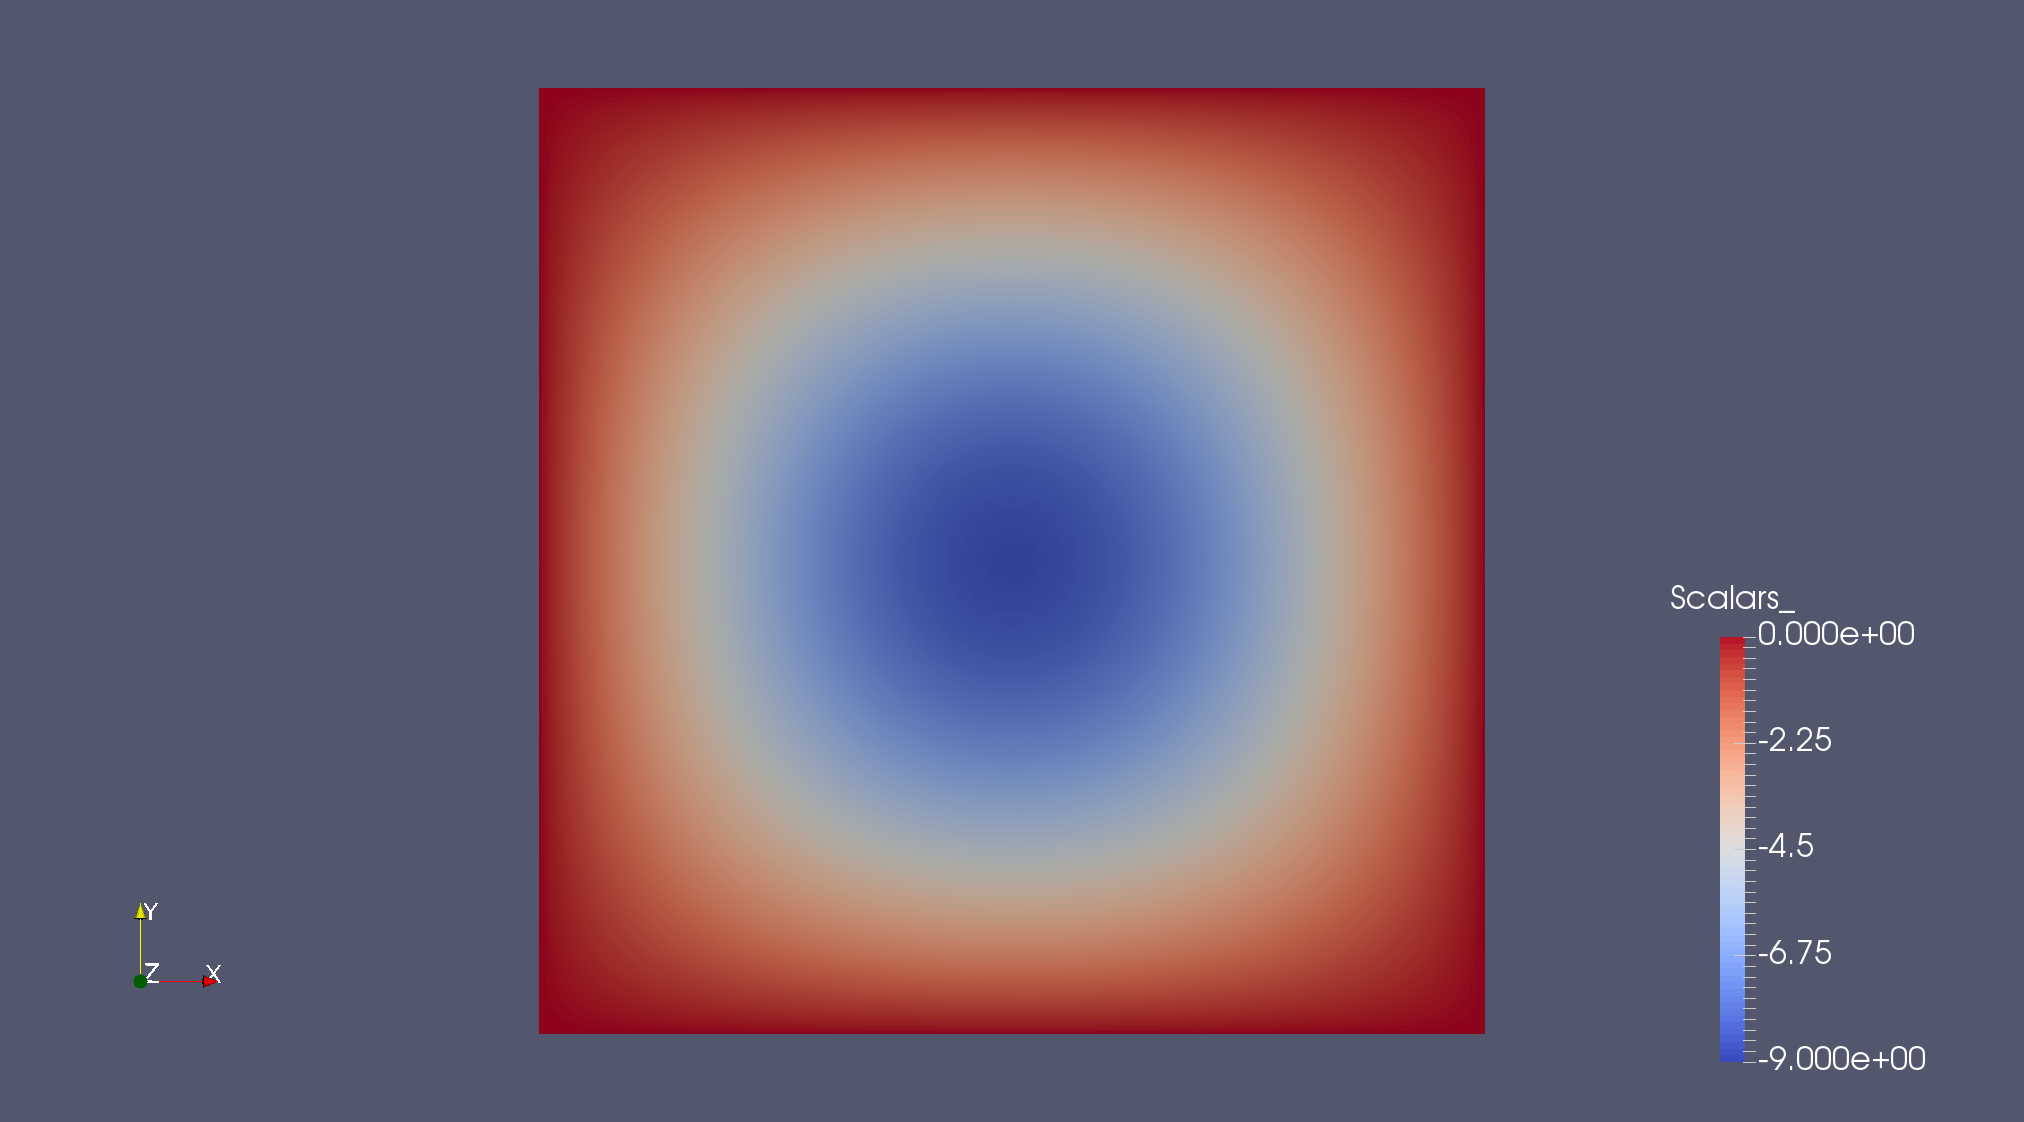
\includegraphics[width=\textwidth]{../thesis/Images/symm-3r-y-0t.png}
\end{center}
\end{frame}

\begin{frame}
State $y$ at $t = T$:
\begin{center}
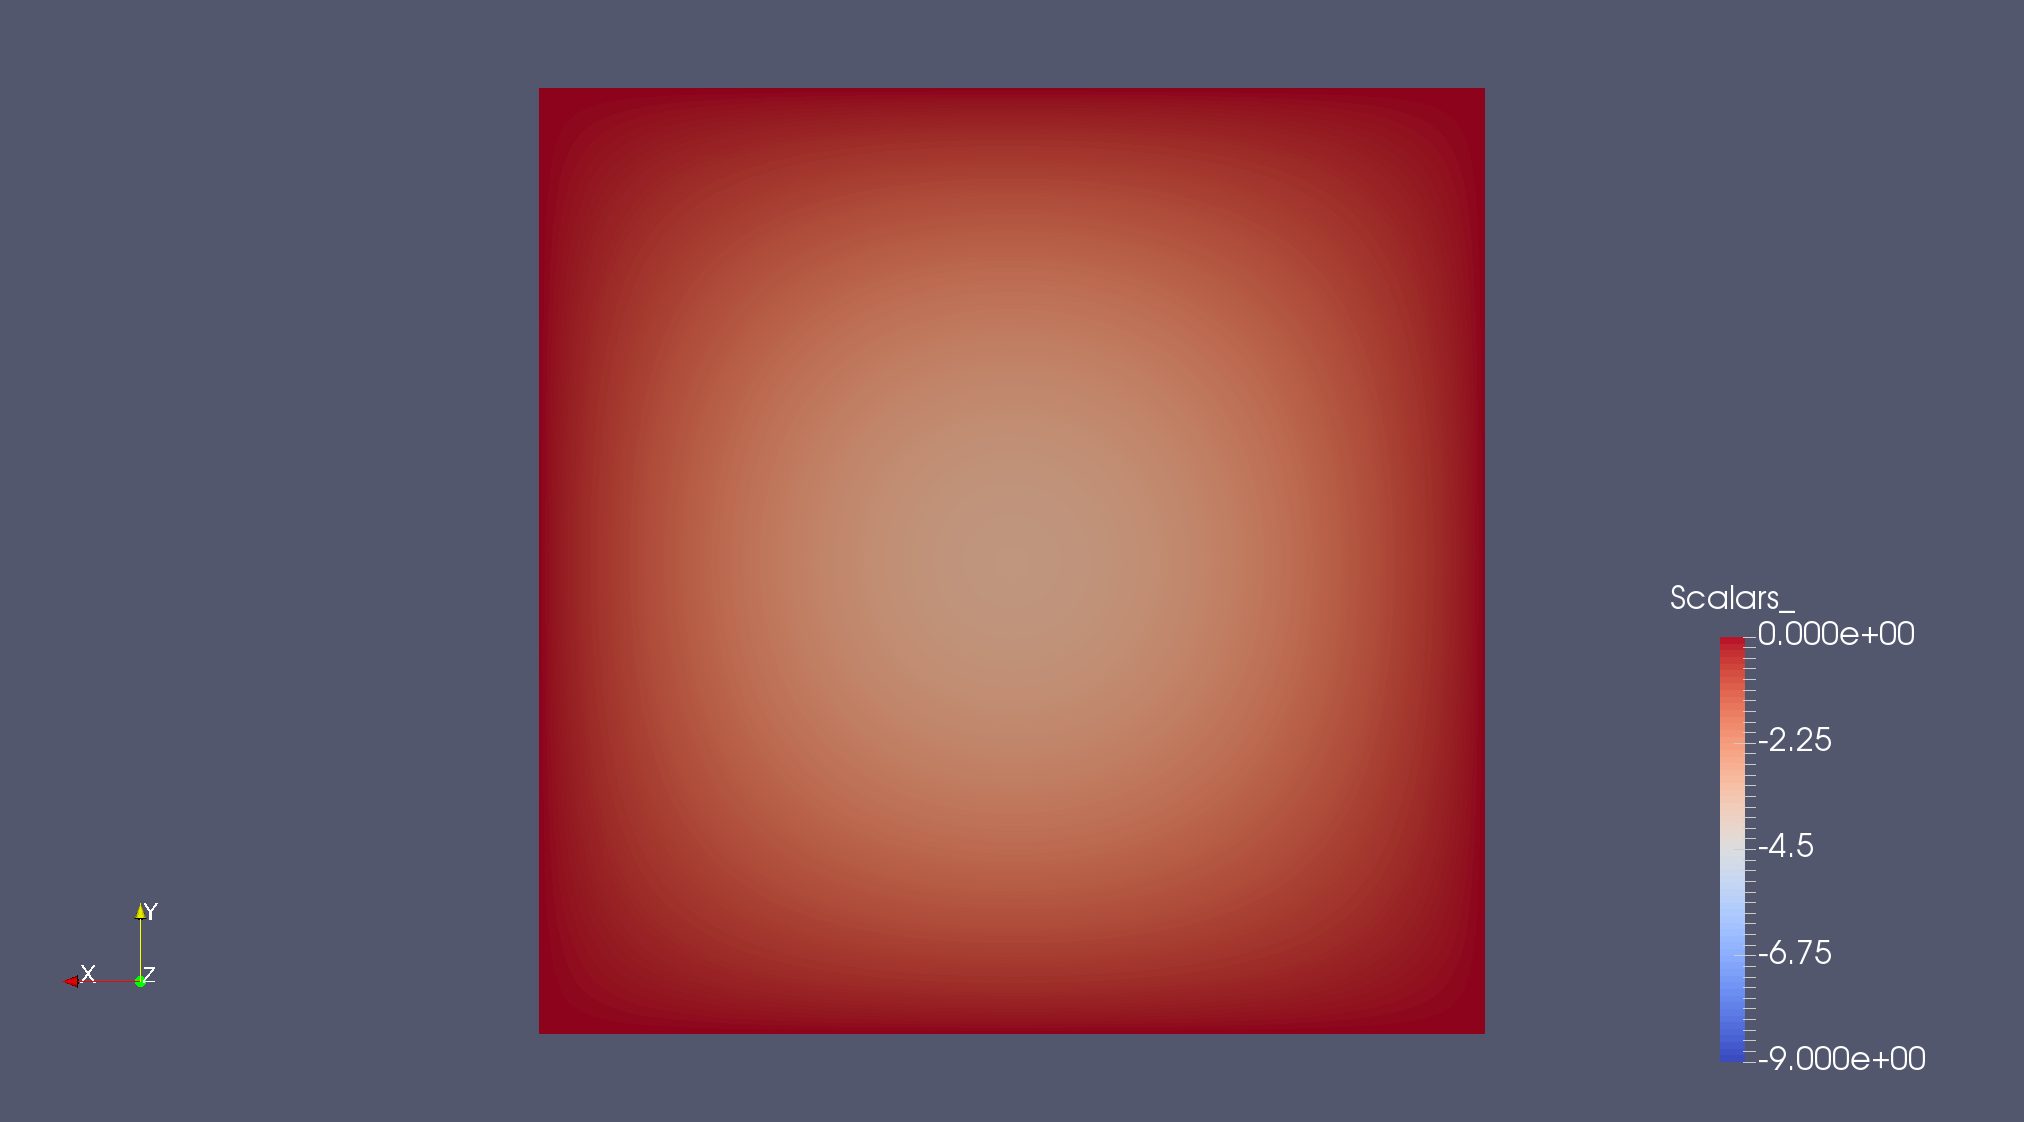
\includegraphics[width=\textwidth]{../thesis/Images/symm-3r-y-Tt.png}
\end{center}
\end{frame}

\begin{frame}
Control $u$ at $t = 0$ ($t = T$ is constantly zero due to initial conditions):
\begin{center}
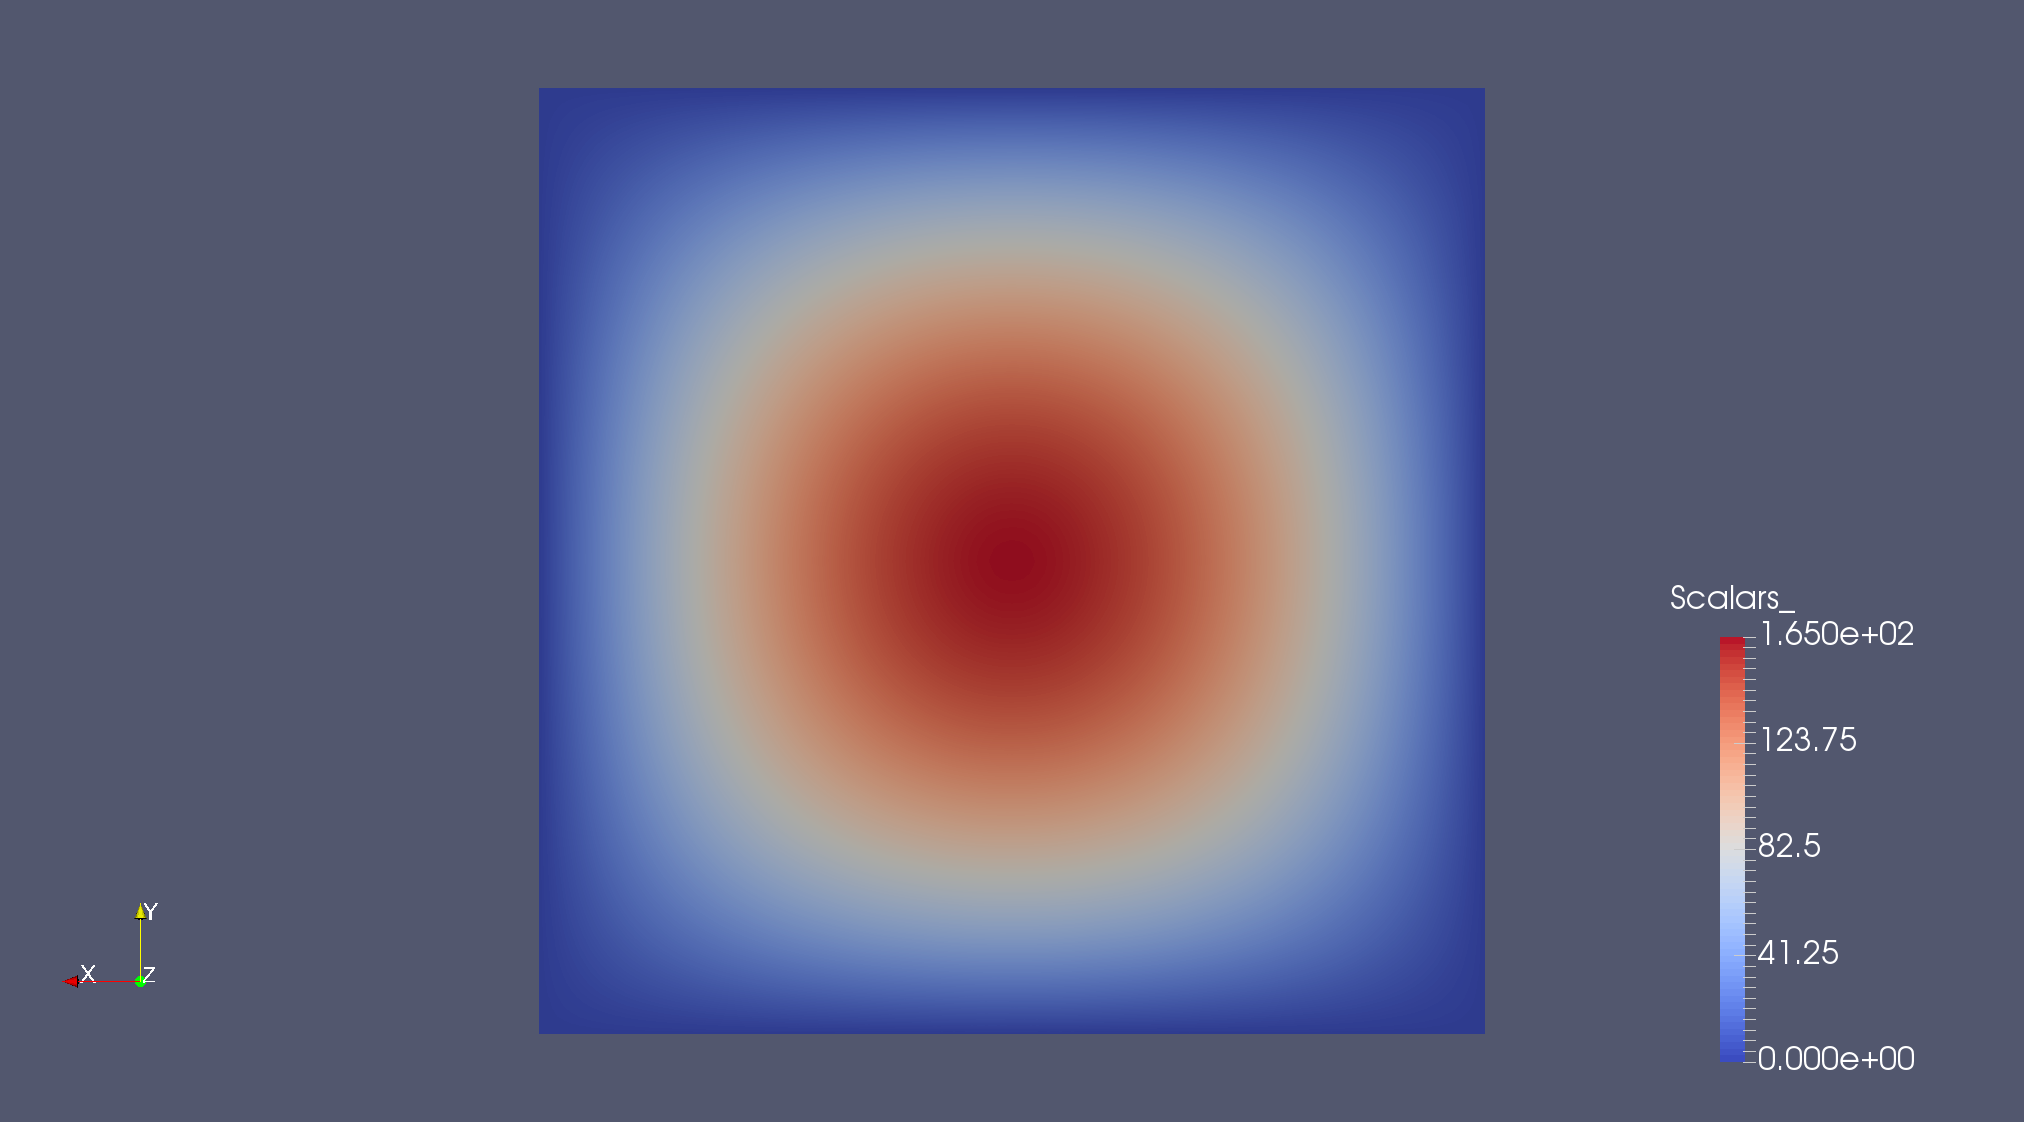
\includegraphics[width=\textwidth]{../thesis/Images/symm-3r-u-0t.png}
\end{center}
\end{frame}

\subsection{Constrained and unconstrained examples}

\begin{frame}
\begin{itemize}
\item Setup: $\Omega = [0, 1]^2$, $T = 1$, $\lambda = 0.1$. $y_0 \equiv 1$, $y_\Omega \equiv 40$.
\item State and control are rotationally symmetric, thus $u$ is shown at $\{ 1 \} \times [0, 1] \times [0, T]$.
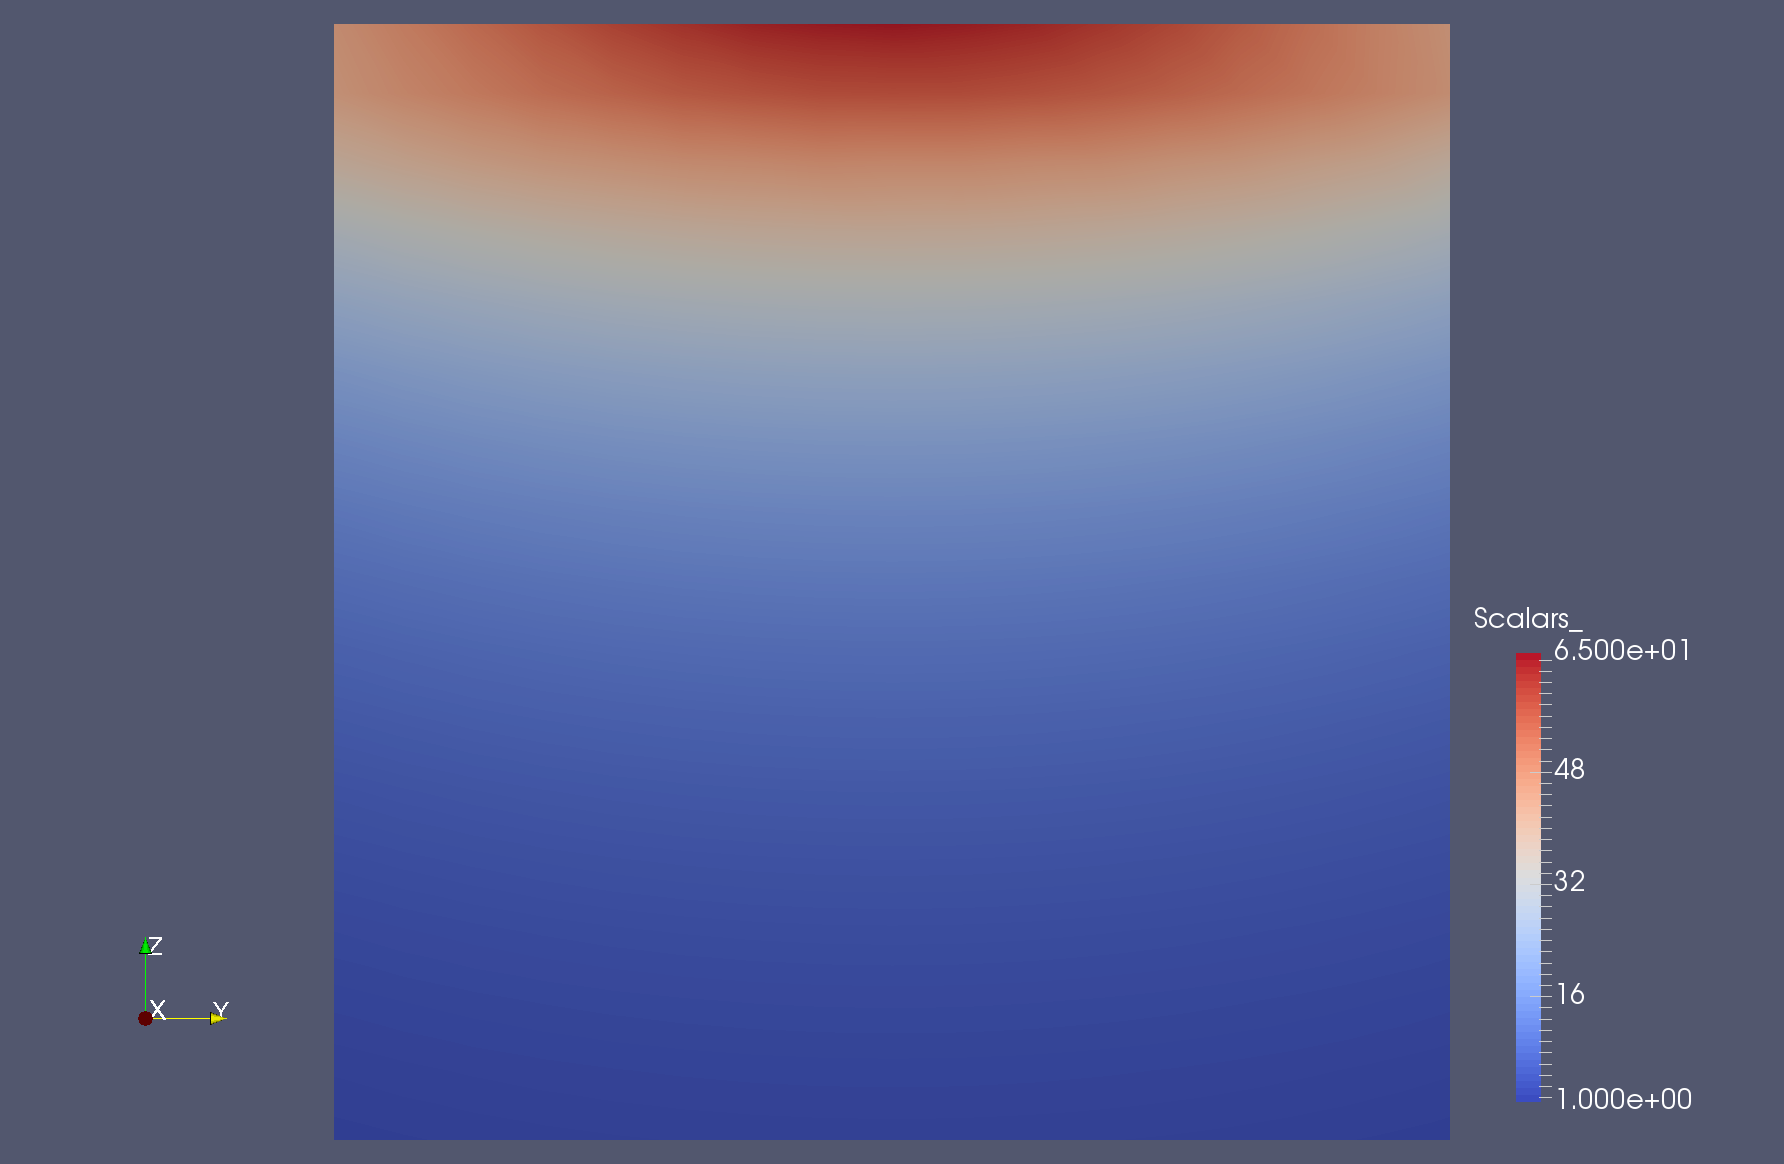
\includegraphics[width=0.9\textwidth]{../thesis/Images/boundary-const-u.png}
\end{itemize}
\end{frame}

\begin{frame}
State at $t = T$:
\begin{center}
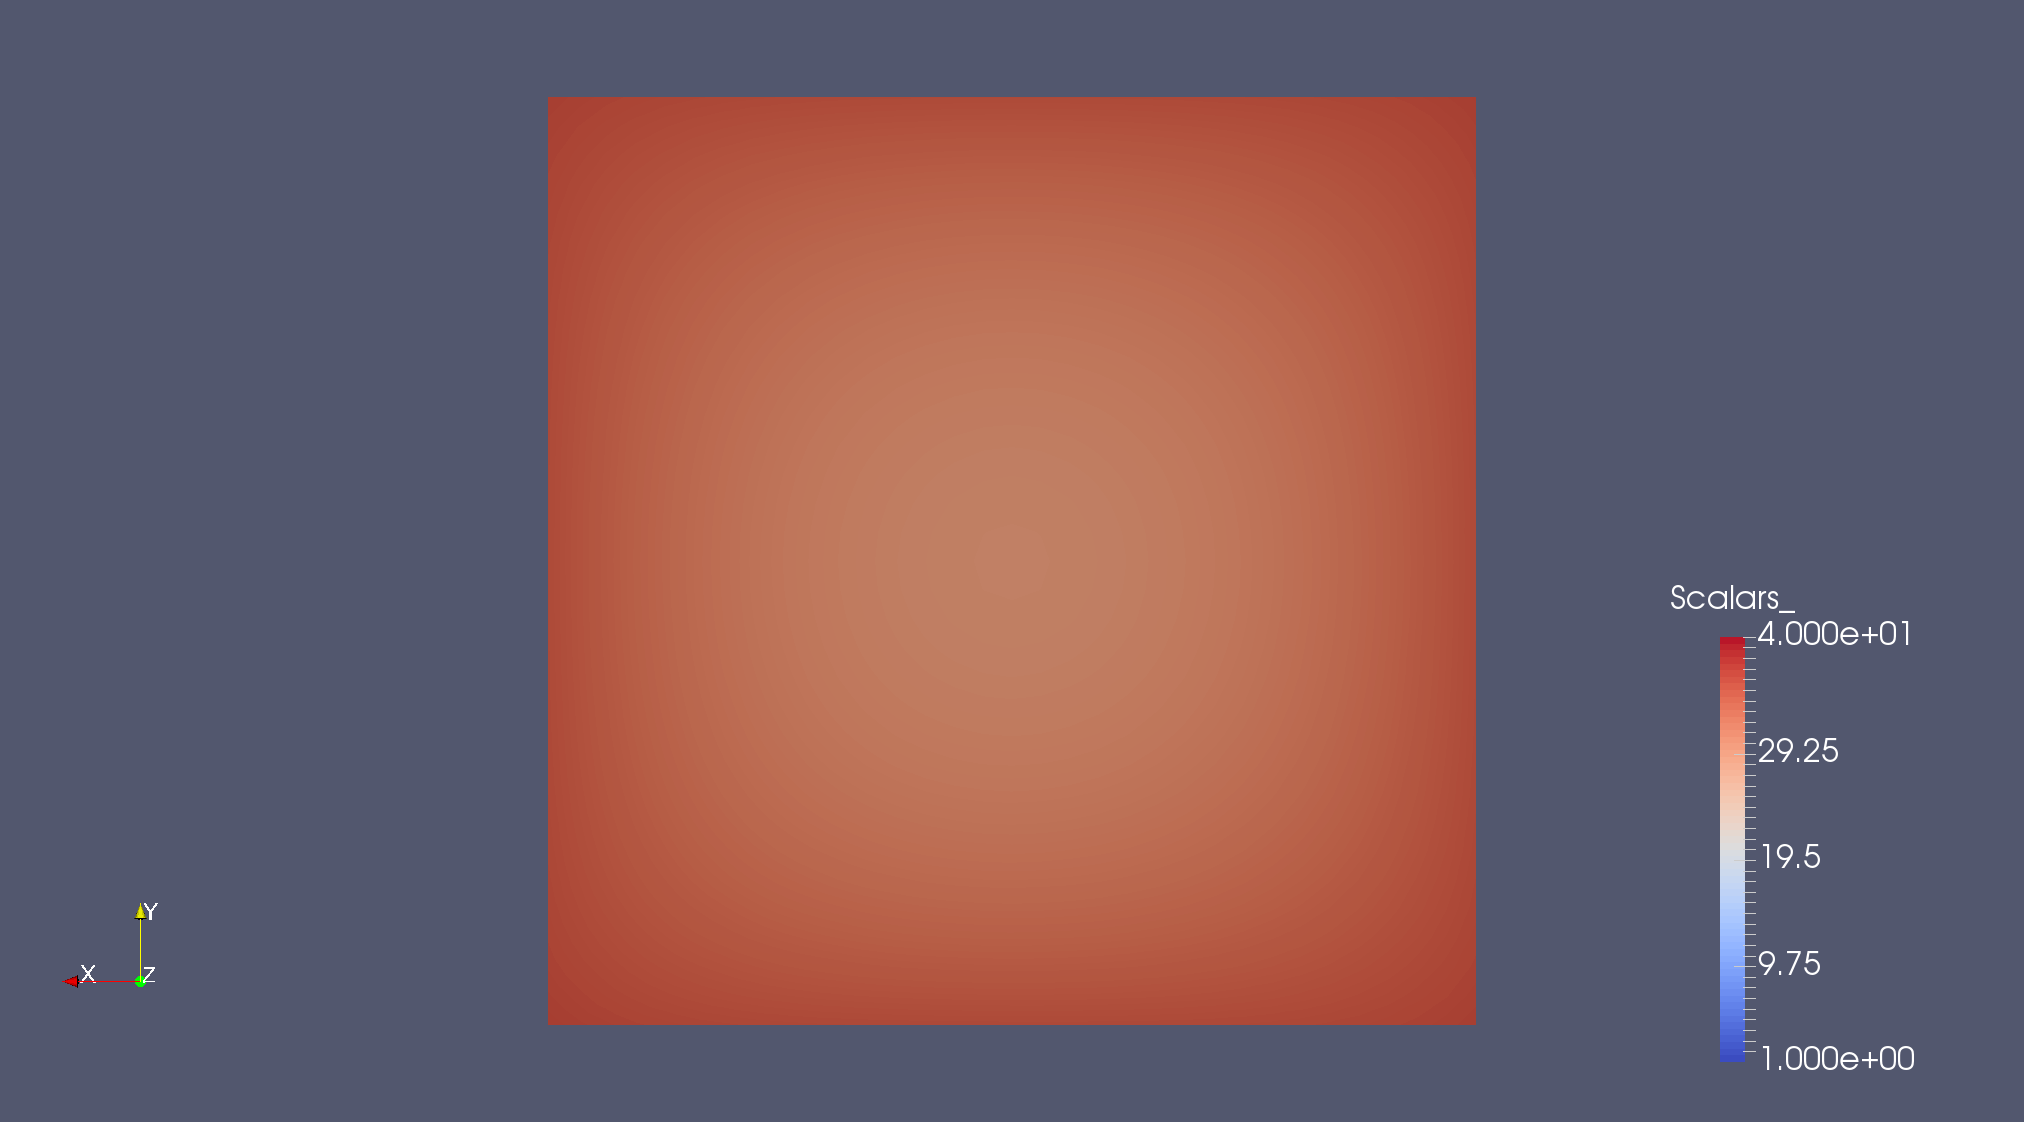
\includegraphics[width=0.9\textwidth]{../thesis/Images/boundary-const-y-endtime.png}
\end{center}
\end{frame}

\begin{frame}
Same setup with the restrictions $10 \geq u(x, t) \geq 40$:
\begin{center}
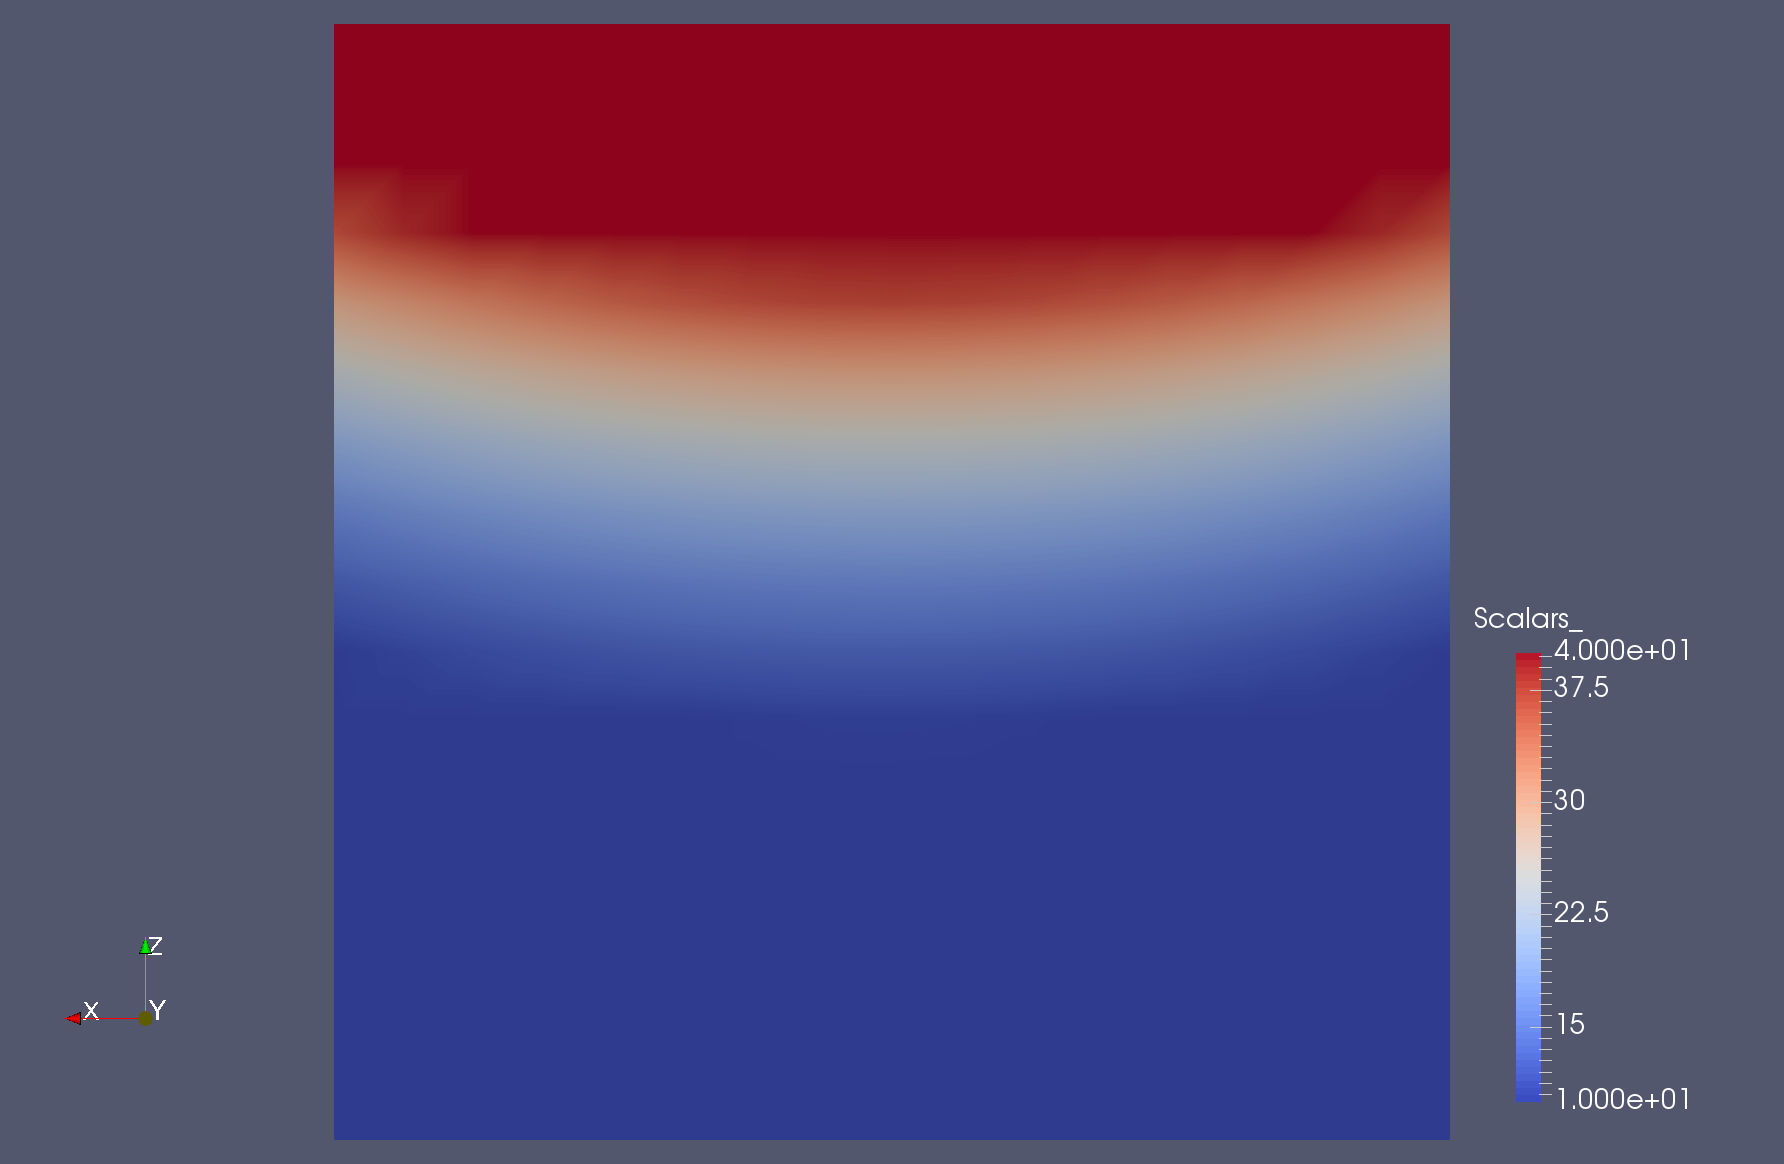
\includegraphics[width=0.9\textwidth]{../thesis/Images/boundary-cont-u-rest.png}
\end{center}
\end{frame}

\begin{frame}
State of the restricted control at $t = T$:
\begin{center}
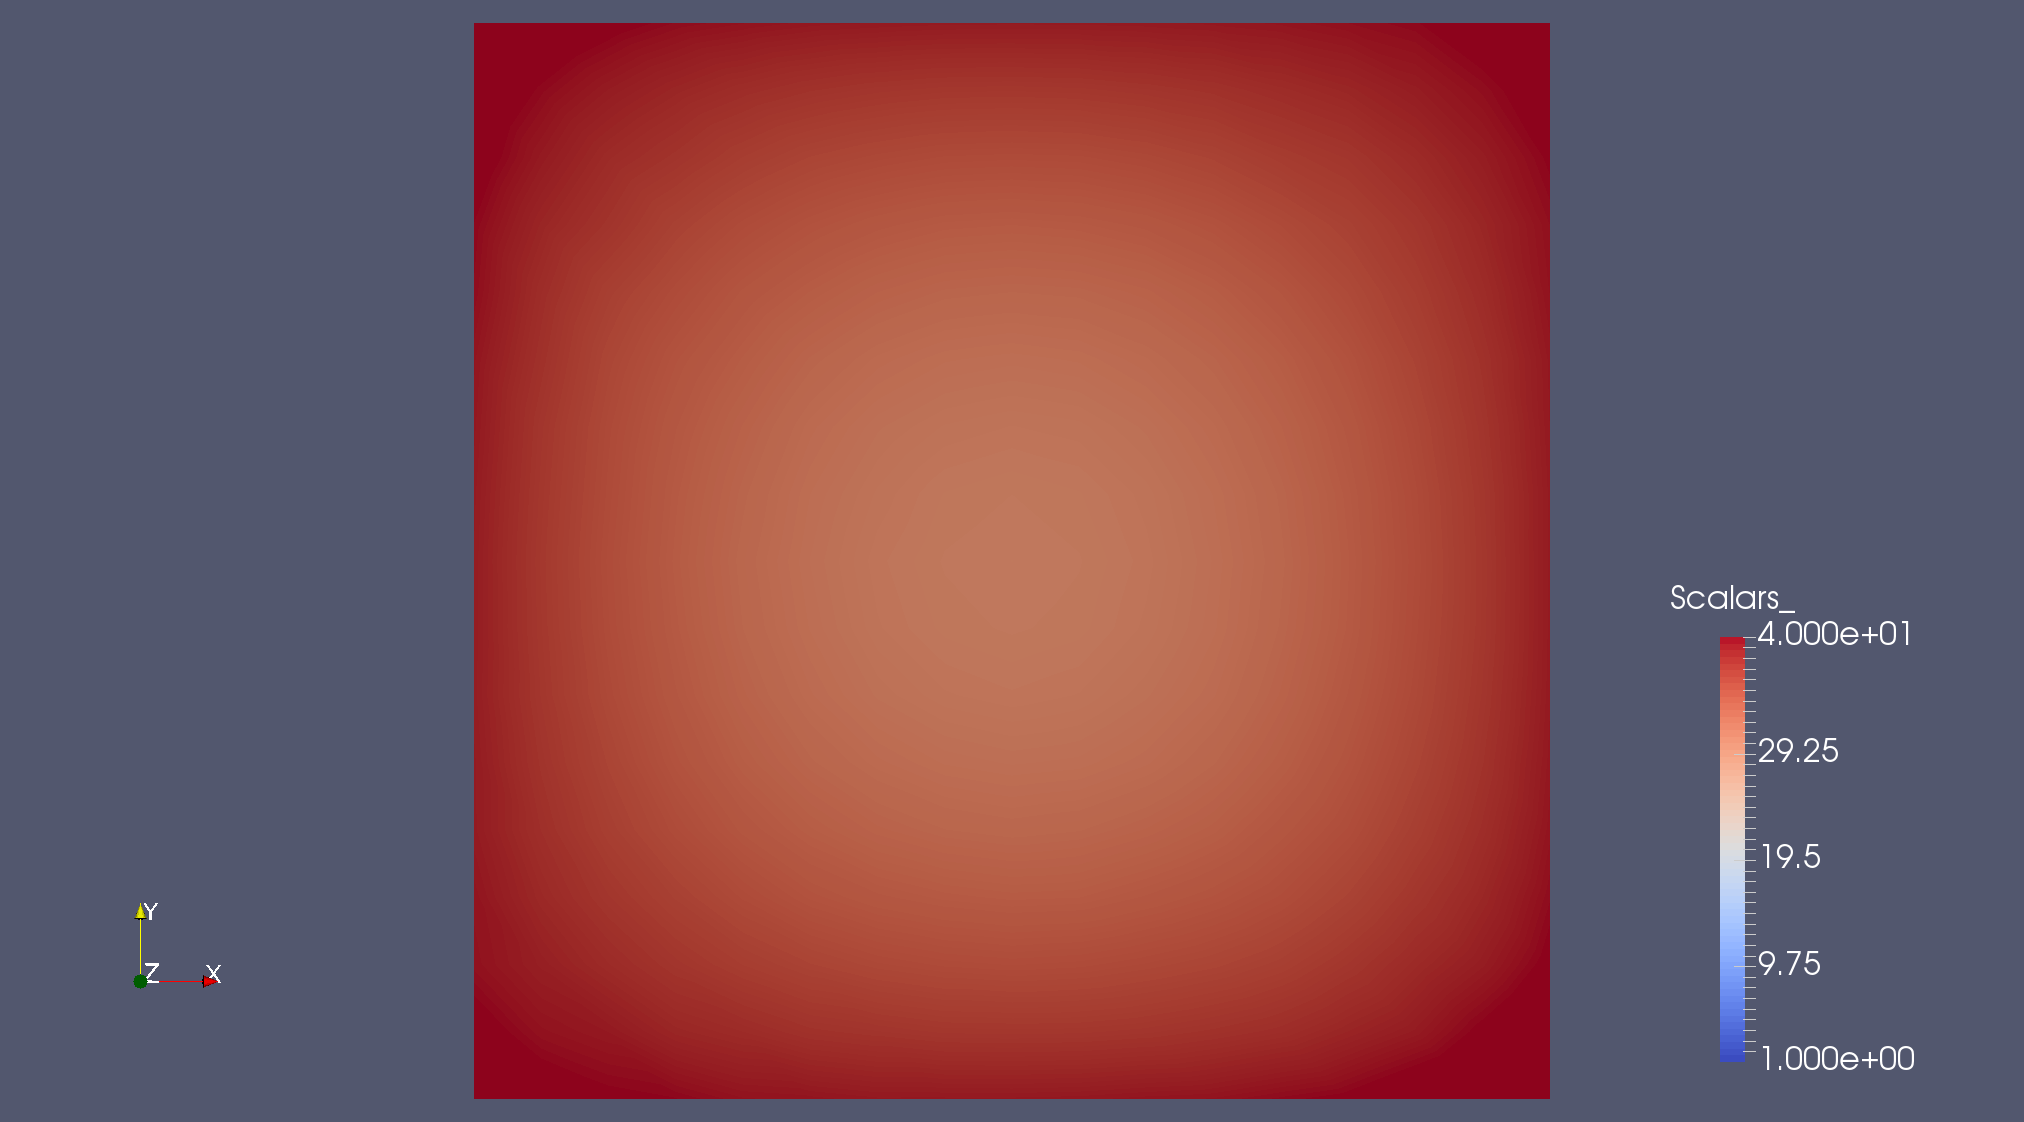
\includegraphics[width=0.9\textwidth]{../thesis/Images/boundary-cont-y-rest.png}
\end{center}
\end{frame}

% \begin{frame}
% \begin{thebibliography}{9}

% \end{thebibliography}
% \end{frame}

\end{document}